\documentclass{article}


\usepackage[utf8]{inputenc}
\usepackage{graphicx}
%\usepackage{biblatex}
%\addbibresource{ref.bib}


\renewcommand{\thesubsection}{\thesection.\alph{subsection}}

\author{s316620 
	\\ }

\title{\textbf{Assignment 4}\\
	\\ Longest Prefix match in Routing tables,
	\\ Limitations of Static Routing \& RIP \\}

%\institute{Oslo and Akershus University College of Applied Science}

\date{September 16, 2016}

\begin{document}

\maketitle
\newpage

\part*{Introduction}
\section*{}
The goal of this assignment is to have a short recap into traditional subnetting as well as
VLSM (variable length subnet masks). In this assignment we learn more about routing, particularly the function of routing tables and how the routing tables affect routing decisions.
Furthermore, we explore the limitations of static routing, which is the starting point for grasping the necessity of routing protocol. In the end of the assignment, a simple, basic, IPv4 routing protocol named RIPv2 is being introduced.

\part*{}
\section{Longest prefix match}

\subsection{ What is meant by "Longest Prefix Match" in routing, and what is the 
	function of the subnet mask in each IP address?}


{\textit{Longest Prefix Match}} is the algorithm of choosing the destination while looking for matches in forwarding table. With \textit{Longest Prefix Match}, the entry with the longest prefix are examined first.
That is the entries with the higher subnet mask are matched first. For example if the router's forwarding table has the following two entries:
	\begin{itemize}
	    \item 10.0.2.0/16
	    \item 10.0.2.0/24
	\end{itemize}
Due to the longest prefix match the longer prefix is matched first, i.e. the entry with the subnet mask 24. So the entry 10.0.2.0/24 is checked for a match prior to the other entry with the subnet mask 16. "To resolve ambiguity that can arise when more than one entry matches a destination, Internet forwarding examines entries with the  longest prefix first.\\",%\textcite{LPMcompnet}.\\

The function of the {\textit{Subnet mask}} is to divide the IP address into two parts; one representing the network and the other the host. For example, with the IP address 10.0.11.0/24, the leftmost 24 bits out of 32 bits represent the network and the 8 right bits represents the hosts. 

\textbf{It is also used to find the range of IP address for the hosts in the network, as well as to find the routing}


\subsection{Imagine that a router checks the routing table for information about a particular route and next hop for the 10.10.10.0 network. In the routing table two entries can be found (we are assuming that there is only one routing protocol running on the network subnet mask of 10.10.10.0/16 and next-hop 192.168.1.1 and one entry with a subnet mask of 10.10.10.0/24 and next hop 192.168.1.2. Where will the router forward the packet? Will the router forward the packet to the "192.168.1.1" next-hop or will the router choose the "192.168.1.2" next-hop? Please explain why.}

The router will forward the packet to 192.168.1.2, as discussed in the previous assignment the  longest prefix is matched first which in this case is 10.10.10.0/24 which will return a match.


\subsection{}
The order in which the destination address of a packet is checked against the rules are D,A,C,E,F,B. This is due longest prefix matches first.


\subsection{}
The default route is at entry B, and the default gateway is <e.f.g.h>.



\subsection{The netmask of entry A is 255.255.0.0. What are the netmasks of the other entries?}

The netmask for all the other entries are: \\
\begin{table}[!h]
\begin{tabular}{c|c}
    Entry & Netmask  \\
    B & 0.0.0.0 \\
    C & 255.252.0.0 \\
    D & 255.255.255.240 \\
    E & 255.0.0.0 \\
    F & 248.0.0.0 
\end{tabular}
\end{table}


\subsection{}

\begin{table}[!h]
\begin{tabular}{c|c}
    Dest. address & Nexthop  \\
   10.0.20.17 & <m.n.o.p> \\
   10.0.20.32 & <m.n.o.p> \\
   10.0.20.30 & <m.n.o.p> \\ 
   8.8.8.4 & <u.v.w.x> \\
   7.254.32.45 & <e.f.g.h> \\ 
   9.16.32.79 & <u..v.w.x> \\
   15.0.0.1 & <e.f.g.h> \\
   16.0.0.1 & <e.f.g.h> \\ 
   17.0.0.1 & <e.f.g.h> \\
   10.0.13.2 & <a.b.c.d> \\
   10.1.13.2 & <a.b.c.d> \\ 
   10.3.13.2 & <i.j.k.l> \\ 
   10.4.13.2 & <q.r.s.t> \\ 
   10.5.13.2 & <q.r.s.t> 
   
\end{tabular}
\end{table}



\section{Route selection with subnets, administrative distances and equal routes.}

\subsection{}
If the router got the a packet destined for 192.0.3.150 it would hop to C. This is because C is the nework id for 192.0.3.0/24; range from 192.0.3.1 to 192.0.3.254, 192.0.3.150 is inside this range, and it did not match any other subnet. 

With the destination address 192.0.3.60 the router will forward the packet to B because it matches to 192.0.3.0/26 due to longest prefix match first. 


\subsection{}

\begin{table}[!h]
    \begin{tabular}{|c|c|}
        \hline
        Dest. address & Nexthop \\ \hline
        10.0.1.125    & A       \\ 
        10.0.1.140    & C       \\ 
        10.0.1.200    & D       \\
        \hline
    \end{tabular}
\end{table}

\subsection{}

\begin{table}[!h]
    \begin{tabular}{|c|c|}
        \hline
        Dest. address & Nexthop \\ \hline
        172.25.34.233 & C       \\ 
        10.25.60.12   & A       \\ 
        10.25.48.150  & A       \\
        \hline
    \end{tabular}
\end{table}

\subsection{}

\begin{table}[!h]
    \begin{tabular}{|l|l|}
        \hline
        Dest. address & Nexthop        \\ \hline
        10.3.31.254   & D              \\ 
        10.12.0.80    & A              \\ 
        10.12.0.144   & B              \\ 
        10.3.40.1     & Packet Dropped \\
        \hline
    \end{tabular}
\end{table}


\subsection{}

\begin{table}[!h]
    \begin{tabular}{|l|l|}
        \hline
        Dest. address & Nexthop \\ \hline
        10.0.0.190    & B       \\ 
        10.0.0.182    & D       \\ 
        10.0.0.173    & B       \\
        \hline
    \end{tabular}
\end{table}


\subsection{}
The first routing option with the next-hop c , is where the packet 10.0.10.79 will be sent. because it is directly connected and has the administrative distance of 0.
\subsection{}

\subsection{}

\subsection{}

\subsection{}

\subsection{}

\subsection{}

\subsection{}

\section{Preparation to this assignment based on previous assignments}

\subsection{In assignment 2, you added the following configuration command to Quagga, through the \textit{vtysh} - shell on Choke: "ip route 0.0.0.0/0 10.0.0.1". what was the intention of this command?}

The intention of this command was to add a default forwarding route at Choke for all the default packets to Gateway (10.0.0.1). Thus the next hop for the default packets will be 10.0.0.1 (Gateway). 


\subsection{In assignment 2, you added a command \textit{(that might look similar to the one above)} on the gateway to ensure forwarding of packets destined to Host1. What was the command?}

To ensure the forwarding of packets destined to Host1 from Gateway, I added the command:\\
\textit{ip route 10.0.11.0/24 10.0.0.2}\\
This forwards the packets to Choke(10.0.0.2) which is also connected to the 10.0.11.0/24 subnet.

\subsection{In the previous assignment, you observed a line like \textit{sysctl -w net.ipv4\_forward=1} in \textit{bootlocal.sh} at Choke and Gateway. What is the meaning of this line, and why is it necessary? Which Quagga routing daemons are started in the same script?}

The line : \textit{sysctl -w net.ipv4\_forward=1} is used for enabling IP forwarding at the nodes Choke and Gateway.

This is useful at the router nodes to forward ip address of the different networks.

We also start other Quagga routing daemons in the same script like zebra, modprobe.

\subsection{List out the routing table at Choke, e.g. with the \textit{netstat -rn command (or alternatively the route -n command)}.Assume that two packets arrive at the router, one with destination address 128.39.11.15 and the other with destination address 10.0.11.13. Explain how each packet is treated by the routing table, i.e. in which order each rule you listed out is applied, which entries/lines give a match and in which order.}

The routing table at Choke is listed with the command \textit{route -n}, and can be seen in Figure \ref{3d-choke-route}. 

\begin{figure}[!h]
    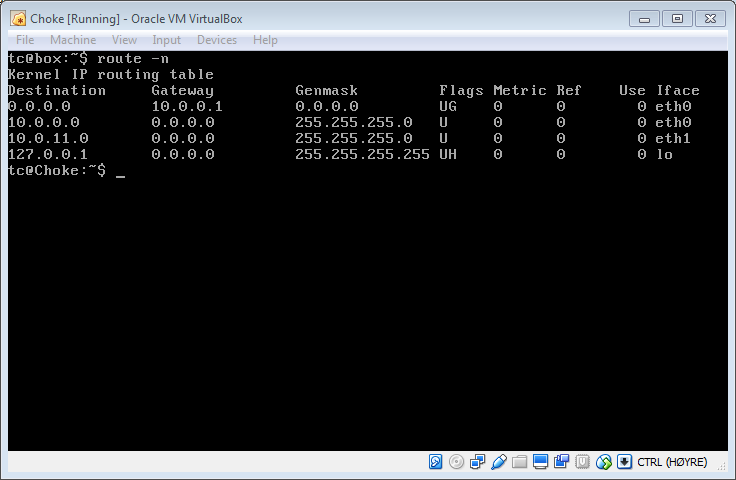
\includegraphics[scale=0.5]{3d-choke-route.png}
    \caption{Choke \textit{route -n}}
    \label{fig:3d-choke-route}
\end{figure}

The packets that arrives with the two destination address 128.39.11.15 and with the destinaiton address 10.0.11.13. In the routing table the first packet with address 128.39.11.15 will be matched with the first rule that is the default gateway and so goest to the node gateway and then to the  internet.

\subsection{}
Done

\subsection{}
Making a clone of the choke with reinitialized MAC addresses, naming it "Router1". 


\subsection{}

Powering on Router1 and the erasing all static IP routing and addresses for the interface inherited from Choke. The \textit{/usr/local/etc/quagga/zebra.conf} file is edited by deleting all the configurations except \textit{password quagga} line. The changes are saved persistently and then powering off. 

\subsection{}
Now making new clones of Router1 calling them Router2 and Router3, and a clone of Host1 calling it Host2. All the clones are have a reinitialized MAC addressess. 

\section{More static routing}

\subsection{}

In the VirtualBox GUI, configuring the adapters of Host2, Router1 and Choke and configuring it to look like the Figure \ref{fig:4-network-topology}. I update the IP addresses in the host and nodes by using Quagga and configure it to the specification in Figure\ref{fig:4-network-topology}. The IP address in Host2 will be configured using the \textit{bootlocal.sh} file. All the IP addresses are assumed to have a 24 bit network mask unless specifically specified in the assignment. 

\begin{figure}[!h]
    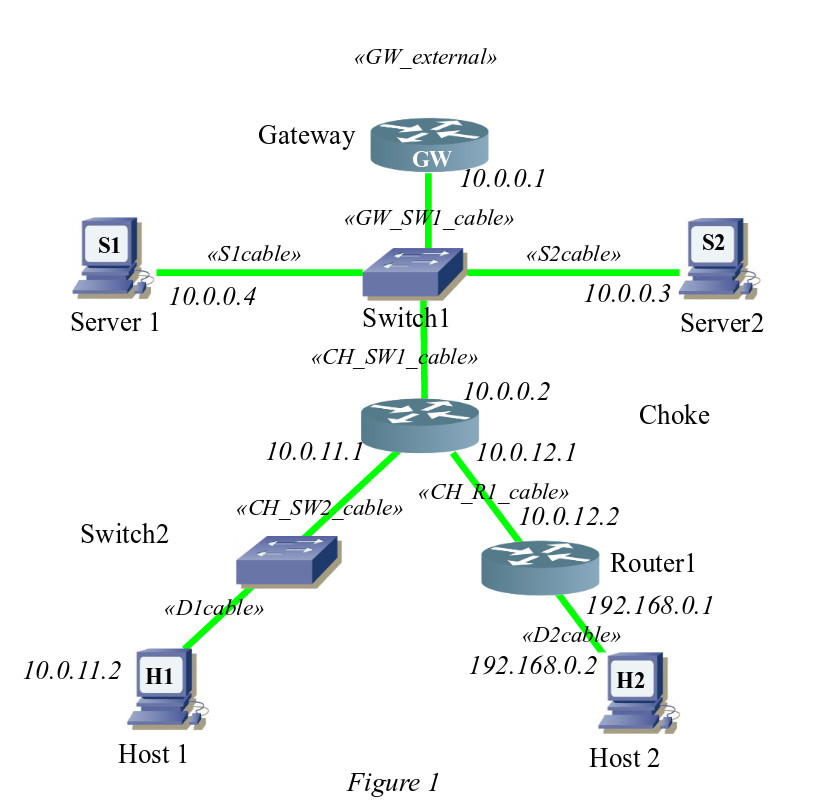
\includegraphics[scale=0.3]{4-network-top.png}
    \label{fig:4-network-topology}
    \caption{Network Topology, Figure 1 in Assignment 4}
\end{figure}

\subsection{}

Now changing the route configuration is important to establish connection between all the hosts. I update the static routes in the routers to have correct packet forwarding. I update the following routers: 
\begin{itemize}
    \item Router1
        \subitem For Router1 we add a default route with Choke as the gateway.
    \item Choke 
        \subitem For Choke we have the routes seen in Figure {\ref{fig:4-choke-route}}.
        That is I have added a route for the packets with destination 192.168.0.0/24, the gateway 10.0.12.2 (Router1). 
        \subitem For Gateway we forward all packets for the destination networks 10.0.12.0/24 and 192.168.0.0/24 to the gateway 10.0.0.2.
\end{itemize}

\begin{figure}[!h]
    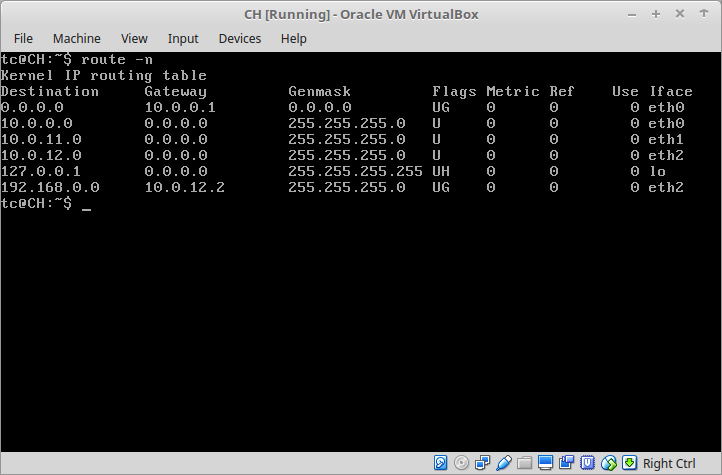
\includegraphics[scale=0.4]{4-choke-routing-table.png}
    \label{fig:4-choke-route}
    \caption{Routing table for Choke (\textit{route -n})}
\end{figure}

\subsection{}
Then to check the connectivity of the network I ping Host1 and the Internet from Host2, as seen in Figure {\ref{fig:4-host2-pinging}}, and Host2 and the Internet from Host1. The ping is successful.

\begin{figure}[!h]
    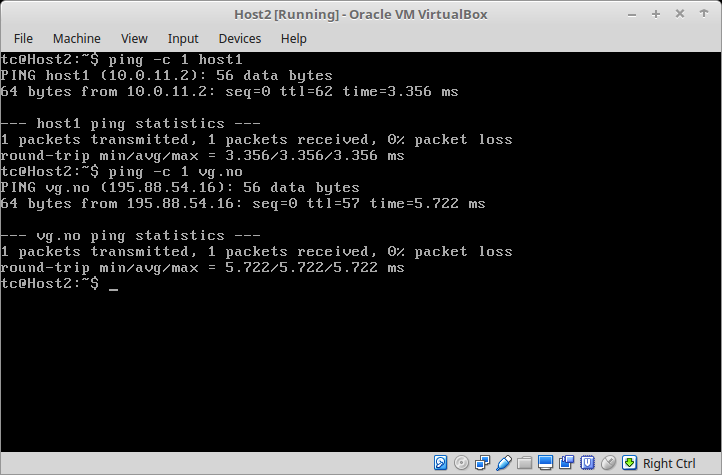
\includegraphics[scale=0.5]{4-host2-ping.png}
    \label{fig:4-host2-pinging}
    \caption{Pinging the Internet and Host1 from Host2.}
\end{figure}

\section{The scalability of Static Routing}

\subsection{}
Configuring the network topology to look like Figure {\ref{5-net-top}}. I update the static IP addressing at the nodes, and use Quagga to update the static route configuration at Router2 (However, I edit the \textit{zebra.conf} file to update the static route configuration at Router1) as seen in Figure{\ref{5-router2-conf}}.

\begin{figure}[h]
    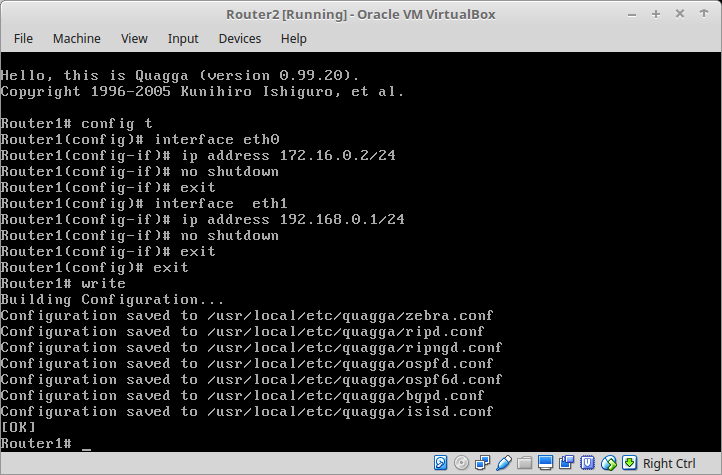
\includegraphics[scale=0.5]{5-router2-quagga-conf.png}
    \label{fig:5-router2-conf}
    \caption{Configuring IP addresses using Quagga (\textit{sudo vtysh})}
\end{figure}


All the routing tables can be seen in the Figures {\ref{fig:5-gateway-route}}, \ref{fig:5-choke-route}, \ref{fig:5-router1-route} and \ref{fig:5-router2-route}.

\begin{figure}[h]
    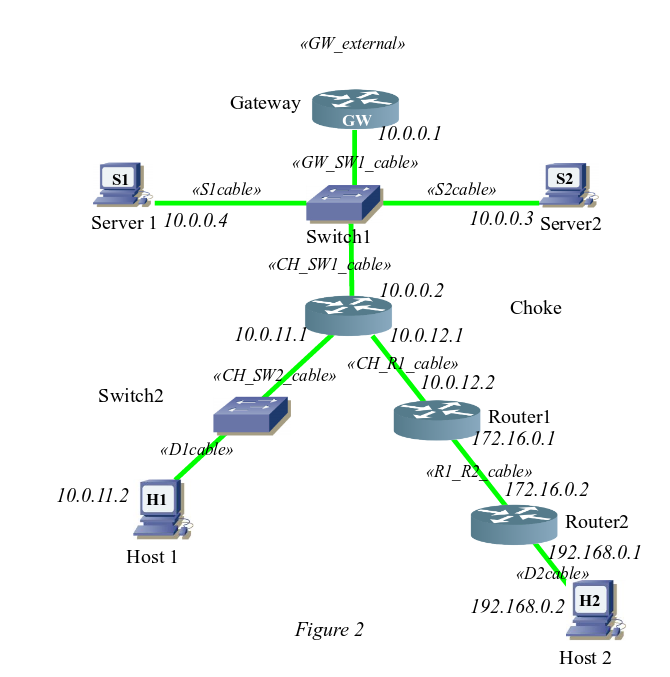
\includegraphics[scale=0.4]{5-net-topo.png}
    \label{fig:5-net-top}
    \caption{Network configuration from Assignment 4}
\end{figure}

\begin{figure}[h]
    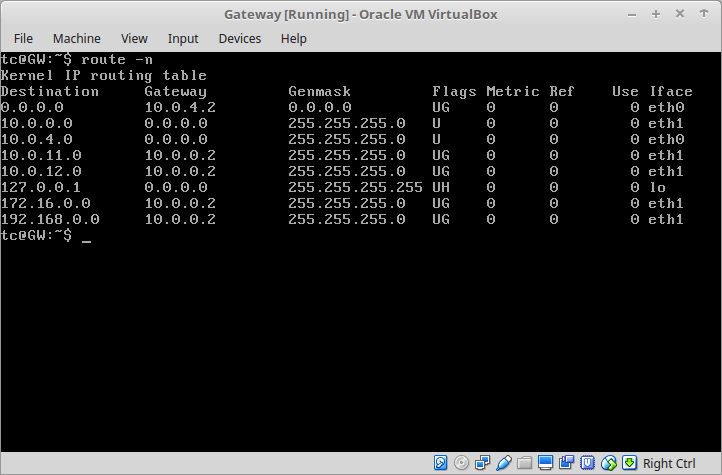
\includegraphics[scale=0.4]{5-gateway-routing.png}
    \label{fig:5-gateway-route}
    \caption{Routing table for Gateway}
\end{figure}

\begin{figure}[h]
    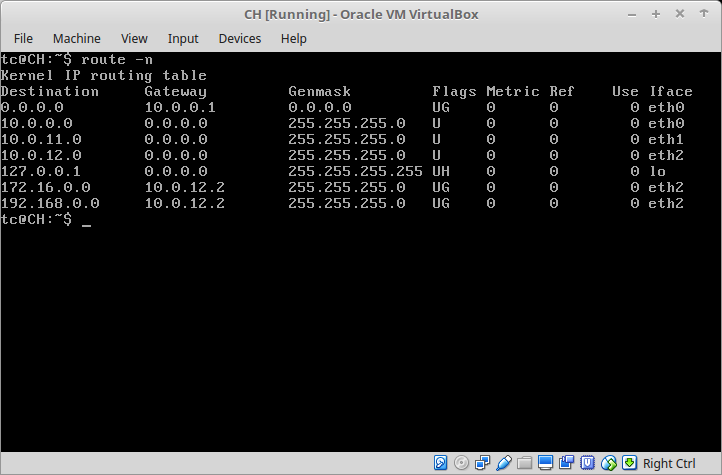
\includegraphics[scale=0.4]{5-choke-routing.png}
    \label{fig:5-choke-route}
    \caption{Routing table for Choke}
\end{figure}

\begin{figure}[h]
    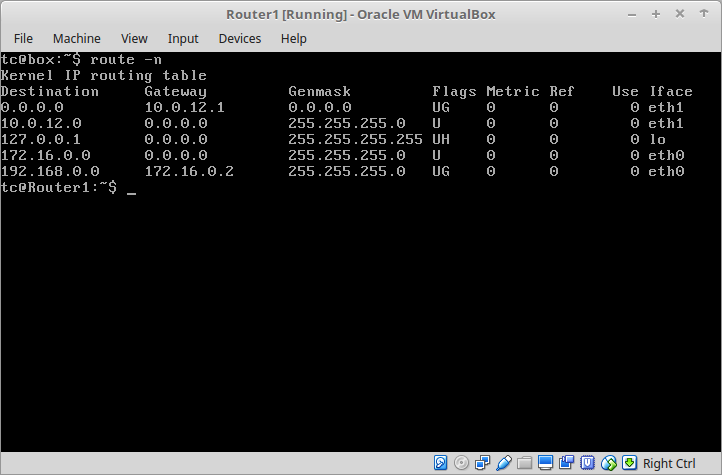
\includegraphics[scale=0.4]{5-router1-routing.png}
    \label{fig:5-router1-route}
    \caption{Routing table for Router1}
\end{figure}

\begin{figure}[h]
    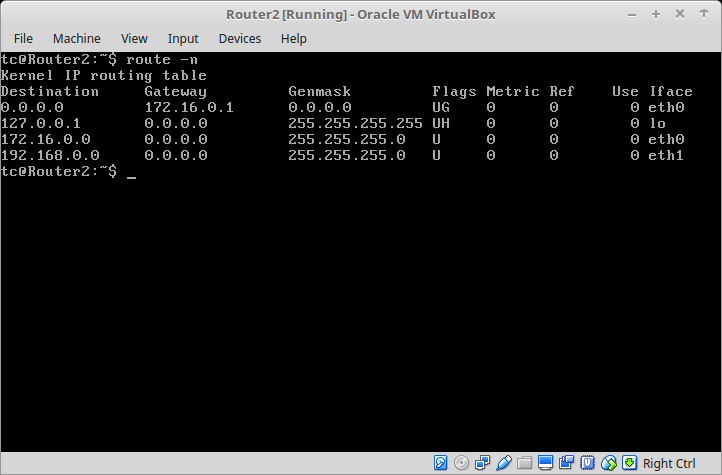
\includegraphics[scale=0.4]{5-router2-routing.png}
    \label{fig:5-router2-route}
    \caption{Routing table for Router2}
\end{figure}


\subsection{}

\subsection{}


\section{Exploring routing protocols in Quagga}

\subsection{} 
Setting up adapters of Router3. Attaching Adapter1 to \"R1\_R3\_cable\", Adapter 2 to \"R2\_R3\_cable\" and adding Adapter 3 and connecting it to "Wireless\_access\_cable". 

\subsection{}
Powering up the router and configuring the IP addresses.
The setup used is shown in the Figure{\ref{fig:6-net-top}}. 

\begin{figure}[h]
    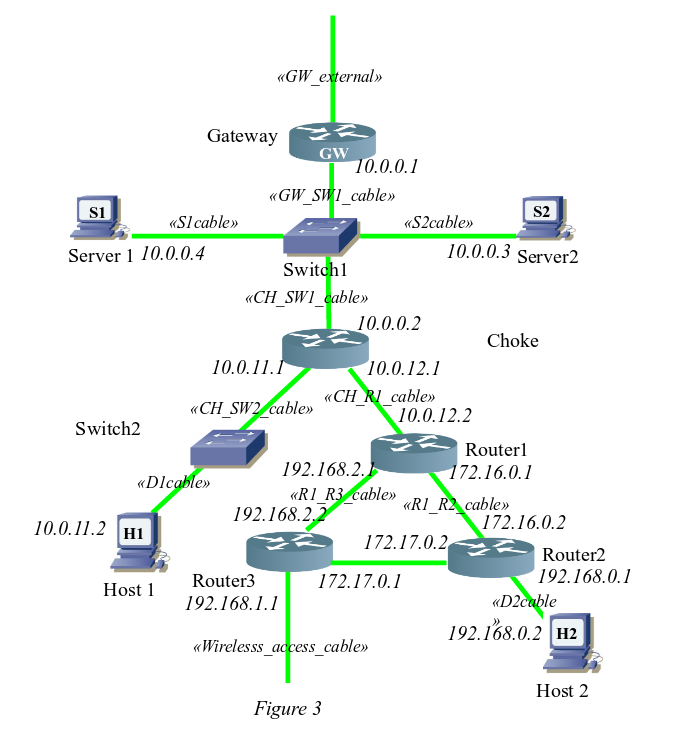
\includegraphics[scale=0.3]{6-network-top}
    \label{fig:6-net-top}
    \caption{Network Topoolgy as shown in Assignment4 Figure 3}
\end{figure}

Now I am configuring the Router3 with RIPv2 routing protocol. 
After the router is configured with its IP addresses. I use the following commands in Quagga( \textit{sudo vtysh}): 

sudo vtysh 
sudo config t 
router rip 
version 2 
network 192.168.2.0/24
network 172.17.0.0/24
network 192.168.1.0/24
exit
exit
write 
exit 

I save the changes persistently. And check the \textit{zebra.conf} and \textit{ripd.conf} file. 


\section{Enabling RIPv2 for your existing topology}



\subsection{}
Next I remove all static routes , except default routes at all the routers. 
This is done by adding "!" sign in front of all "ip route ..." commands in the zebra.conf files.

\subsection{}
Then configuring the RIP as the same way done in Router 3. First I configure gateway to run with the RIPv2 configuraions.Then configuring Choke , Router1 and Router2.The routing tables can se seen in Figure {\ref{fig:routing_tables}}.

\begin{figure}[!h]
    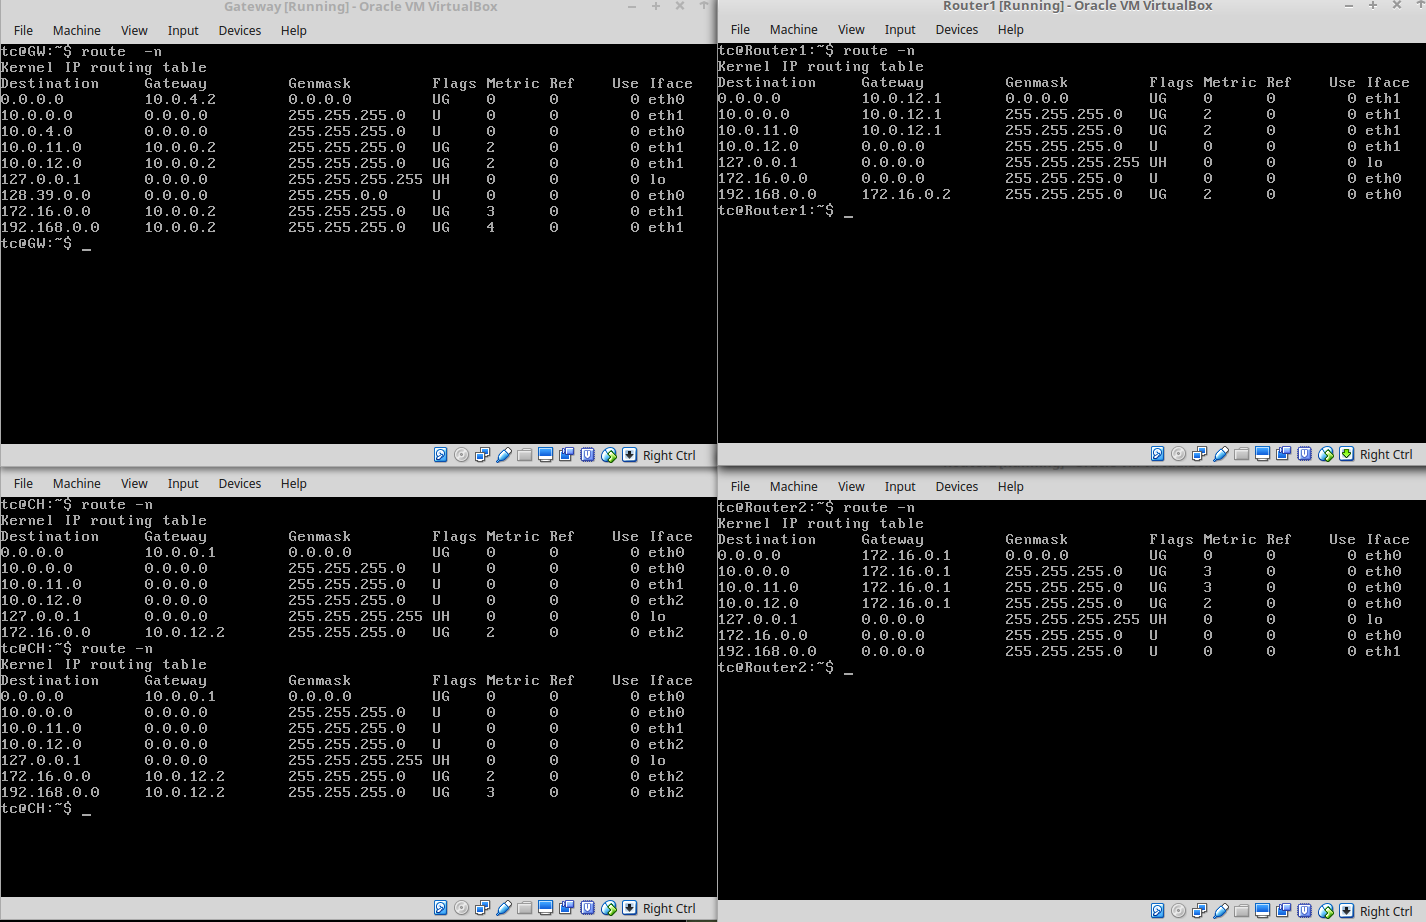
\includegraphics[scale=0.2]{7-routing-tables}
    \label{fig:routing_tables}

    \caption{Routing tables at routers}
\end{figure}

\subsection{}

\subsection{}

\section{Let RIPv2 also set the default routes throughout your sites}

\subsection{}
Removing all the default routes at the \textit{zebra.conf} file and then check that the routers cannot connect outside the network. I did this by pinging outside the network and it failed.

\subsection{} 
Configuring the RIPv2 to distribute the default route instead, by adding the line \textit{default-information originate} at the \textit{ripd.conf} file, before the "network ... ... " line at Gateway.

\subsection{} The connection outside the site have been established and the routing options can be seen in Figure{\ref{fig:router_route}}.

\begin{figure}[h]
    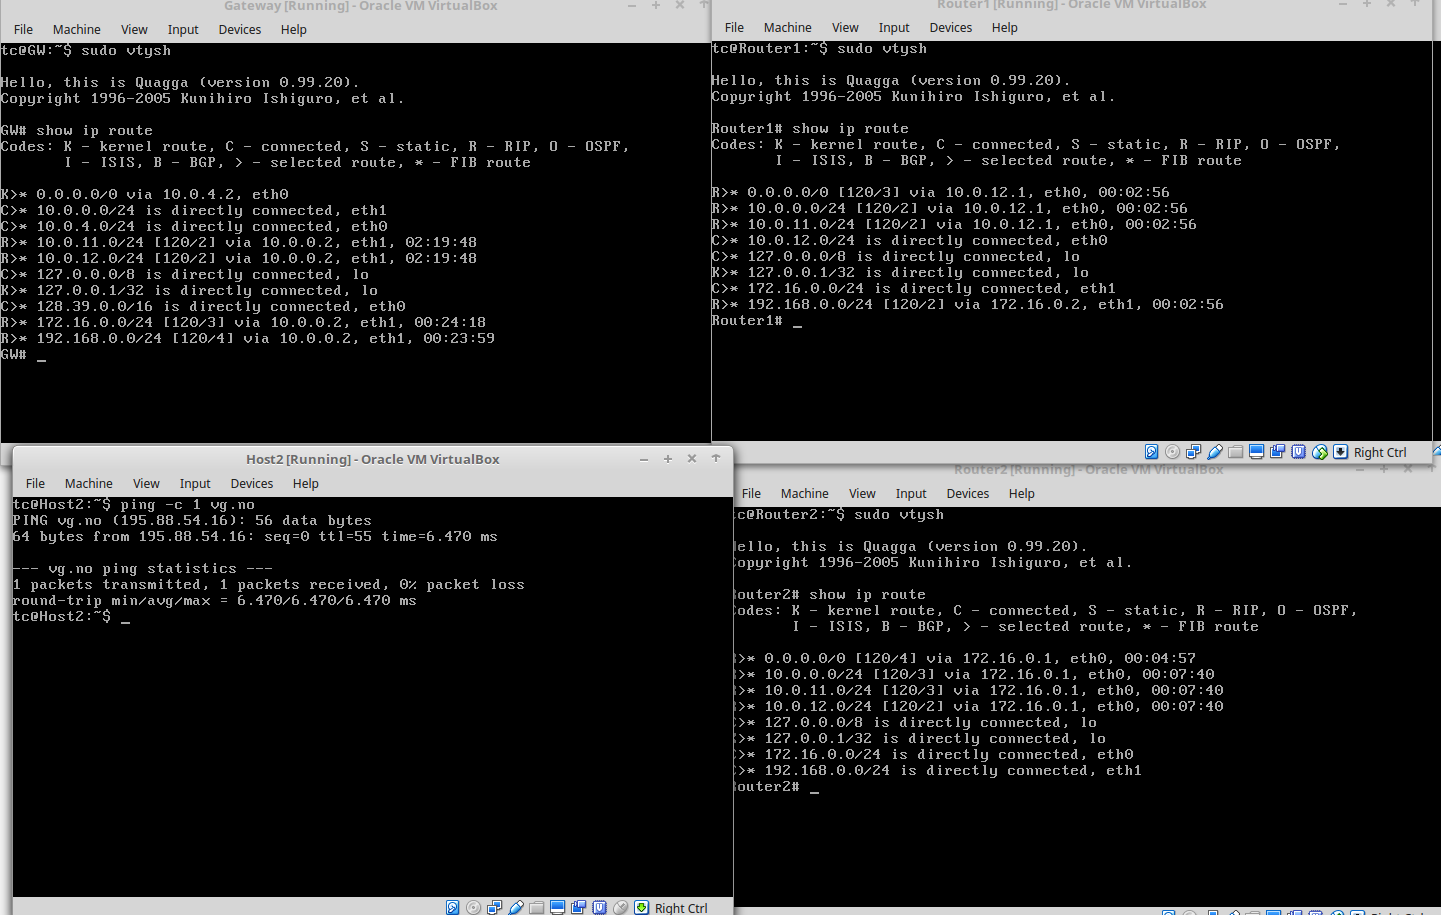
\includegraphics[scale=0.2]{8-router-route}
    \label{fig:router_route}
    \caption{Gateway, Router1 and Router2 routing table and Host2 ping to the internet.}
\end{figure}



\section{Include Router3 in your topology}

\subsection{} 

\subsection{} 
Running traceroute at Gateway seen in Figure \ref{fig:host2-traceroute}
\begin{figure}[!h]
    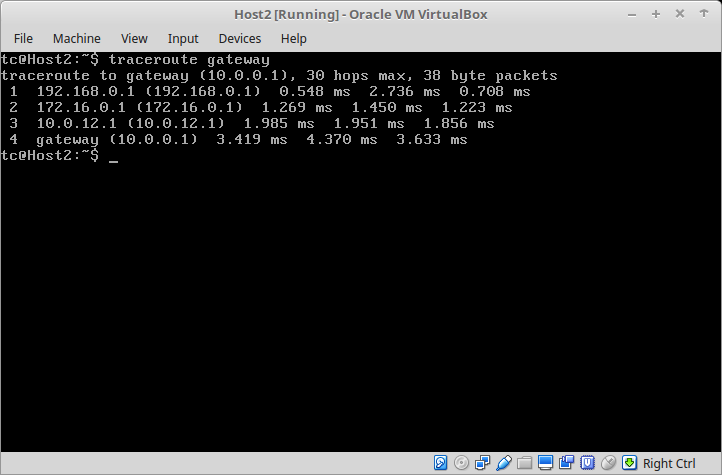
\includegraphics[scale=0.5]{host2-traceroute-gateway}
    \label{fig:host2-traceroute}
    \caption{Running traceroute at Host2}
\end{figure}

\subsection{} 

\section{Documenting your final Quagga (RIP \& Zebra) configuration}

\subsection{} 
The Administrative Distance is running order of the routing source. The lower administrative distance will be choose first. Local routes have the value 0, Static routes 1 and RIP's is 120.
\subsection{}

My ripd.conf files look like this Figure \ref{fig:conffile}.

\begin{figure}[!h]
    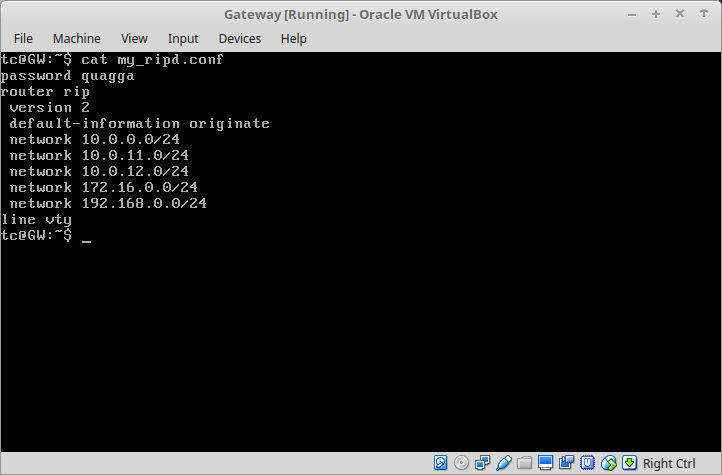
\includegraphics[scale=0.5]{conffile}
    \label{fig:conffile}
    \caption{Ripd.conf file at gateway}
\end{figure}



\end{document}









